%!TEX encoding=UTF-8 Unicode
%!TEX root=../tabarnac.tex

\section{Related Work}
\label{sec:soa}
\begin{figure}[!b]
    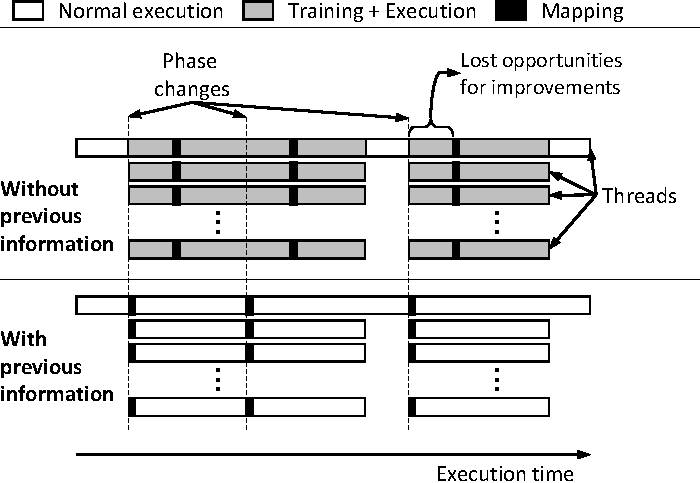
\includegraphics[width=\linewidth]{img/timeline}
\end{figure}

\MD{classify mechanisms}

\subsection{Mapping}
\label{sec:soa-mapping}
\DB{If you can try writing something here, I'll do the next subsection}
\subsection{Profiling}
\label{sec:soa-profiling}

\begin{itemize}
    \item MemProf \cite{Lachaize12MemProf}
        \begin{itemize}
            \item AMD IBS
            \item No nice display, user have to go through complex traces
        \end{itemize}
    \item ``Manual'' characterization \cite{Majo13(Mis)understanding,Jiang14Understanding}

    \item Based on perfcounter no by structures informations, focus and stall
        / cache miss rather than patterns \cite{Bosch00Rivet, Weyers14Visualization}
        => Tells what not why
    \item Node and by page view remote/local access, no structure informatiosn,
        no patterns \cite{Tao01Visualizing}
\end{itemize}


\MD{mechanisms with prior information have highest potential for improvements, but currently:
- lack of information about memory access behavior
- lack of information about ways to improve behavior
}
